\documentclass{ximera}

\title{Autokatalytische reactie: Oefening}
\author{Mila Vervoort}
\license{CC: 0}         % replace with an appropriate license, or set it in xmPreamble

\begin{document}
\begin{abstract}
    Oefening op autokatalytische reactie
\end{abstract}
\maketitle

\section*{Autokatalytische Reacties}

Een \textbf{autokatalytische reactie} is een chemische reactie waarbij één van de producten de reactie versnelt door als katalysator te fungeren. Met andere woorden, de reactie “katalyseert zichzelf”.  

Een typisch voorbeeld van een autokatalytische reactie is:

\[A \rightarrow B\]

Hierbij is \(B\) zowel een product als een katalysator voor de reactie. De reactiesnelheid neemt toe naarmate er meer \(B\) gevormd wordt. \\

De snelheidsvergelijking van deze reactie is:
\[
-r_A = k C_A C_B
\]
waarbij:
\begin{itemize}
    \item \(C_A\) = concentratie van reactant \(A\)  
    \item \(C_B\) = concentratie van product/katalysator \(B\)  
    \item \(k\) = snelheidsconstante
\end{itemize}

De concentratie van B kan herschreven worden als:
\[
C_B = C_{B0} + C_{A0} - C_A
\]

Invullen in de snelheidsvergelijking geeft:

\[
-r_A = k C_A (C_{B0} + C_{A0} - C_A)
\]


Dit kan ook verder uitgeschreven worden in functie van conversie met $C_A = C_{A0}(1-X_A)$:
\[
-r_A
= k C_{A0}(1-X_A)(C_{B0} + C_{A0}X_A)
\]
\begin{remark} \
 \begin{itemize}
     \item Indien er aanvankelijk geen product aanwezig is:
     \[-r_A = k C_A (C_{A0}-C_A)\] 
     \item Indien $C_{B0}=\varepsilon >0$:
     \[-r_A = k C_A (\varepsilon + C_{A0}-C_A)\]
     of in conversievorm:
 \end{itemize}
 \end{remark}

Hoe kunnen we deze autokatalytische reacties drijven tot een zeer hoge conversie? 

We veronderstellen:
\begin{itemize}
\item isotherme werking
\item ideale reactoren
\item constante densiteit
\end{itemize}

Een autokatalytische reactie heeft geen monotoon stijgende kinetiek.
De reactiesnelheid vertoont een maximum bij een intermediaire
concentratie (of conversie). Hierdoor veranderen ook de relatieve
prestaties van verschillende reactoren.

De verblijftijd wordt gegeven door:
\[
\tau_{\text{CSTR}} 
= \frac{X_A}{-r_A/C_{A0}\big|_{X_A}}
\] 

\[
\tau_{\text{PFR}} 
= \int_{0}^{X_A} \frac{dX_A}{-r_A/C_{A0}}
\]
Bij monotoon stijgende kinetiek geldt steeds:
\[
\tau_{\text{CSTR}} > \tau_{\text{PFR}}
\]
Een PFR is dan altijd volume-efficiënter.

Bij een autokatalytische reactie is dit echter
niet langer gegarandeerd. Omdat de reactiesnelheid
bij lage conversie zeer klein is (weinig product aanwezig),
werkt een PFR in het begin van zijn lengte in een
ongunstig kinetisch gebied.
Een CSTR daarentegen opereert volledig aan de
uitlaatconcentratie. Indien deze zich dichter bij
het snelheidsmaximum bevindt dan de lage
inlaatconcentratie van een PFR, kan de CSTR
bij lage conversies een kleinere verblijftijd
vereisen dan de PFR.

Met andere woorden:
\begin{itemize}
\item Bij lage conversie kan de CSTR performanter zijn.
\item Bij hogere conversie wordt de PFR opnieuw voordeliger.
\end{itemize}
Dit kan eenvoudig geverifieerd worden door in de
interactieve figuur de gewenste conversie te variëren
en $\tau_{\text{CSTR}}$ en $\tau_{\text{PFR}}$ te vergelijken.
\begin{center}
\geogebra{vrjscbe6}{700}{700}
\end{center}
Autokatalytische kinetiek doorbreekt dus de klassieke
rangorde waarbij een PFR altijd efficiënter is dan een CSTR. 
Ook andere reactorconfiguraties kunnen performanter zijn, en dat wordt duidelijk in volgende oefening.

\subsection*{Gegeven}

\begin{align*}
C_{A0} &= 1 \ \text{kmol/m}^3 \\
C_{B0} &= 0 \\
q &= 10 \ \text{m}^3/\text{h} \\
C_{A,\text{uit}} &= 0.01 \ \text{kmol/m}^3 \\
k &= 4.2 \times 10^{-4} \ \text{m}^3/(\text{kmol}\cdot \text{s})\\
X_A &= 0.99\\
\end{align*}

\subsection*{Gevraagd}

\begin{enumerate}
\item Bepaal het benodigde volume van één CSTR.
\item Bepaal het benodigde volume voor een serieschakeling van: één CSTR gevolgd door één PFR met een intermediaire concentratie
  \[
  C_A = 0.5 \ \text{kmol/m}^3.
  \]
\item Bepaal de optimale recycleverhouding en het vereiste volume voor een PFR met recycle.
\end{enumerate}

\subsection*{Eén CSTR}
\begin{exercise}
Bepaal het benodigde volume van één CSTR. 
$\text{Volume} = \answer{661} m^3$
    \begin{hint}
    Gebruik de formule afgeleid voor de verblijftijd.
    \end{hint}
    \begin{solution}
    \[ \tau = \frac{V}{q} = \frac{C_{A0} - C_{A,\text{uit}}}{k\,C_{A,\text{uit}}\left(C_{A0} - C_{A,\text{uit}}\right)} = 66.1\ \text{uur}\]
    \[V = 661\ \text{m}^3\]
    \end{solution}
\end{exercise}

\begin{exercise}
Bepaal het benodigde volume van een serieschakeling van één CSTR en één PFR met een intermediaire concentratie $C_A^* = 0.5\ \text{kmol/m}^3$ en een eindconversie $X_A = 99\%$.
\begin{question}
    Wat is de beste optie?
    \begin{multipleChoice}
        \choice[correct]{Eerst een CSTR daarna een PFR}
        \choice{Eerst een PFR daarna een CSTR} 
    \end{multipleChoice}
    \begin{solution}
    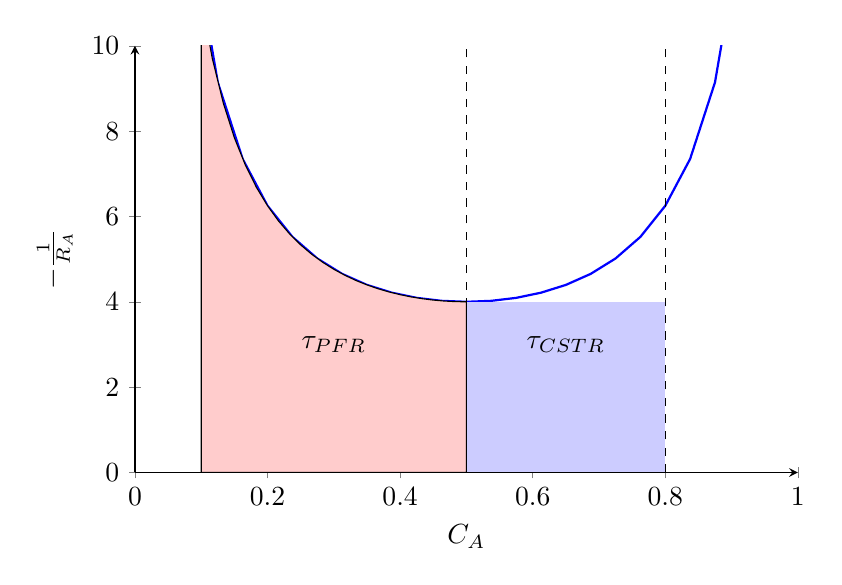
\begin{tikzpicture}
    \begin{axis}[
        width=10cm,
        height=7cm,
        xlabel={$C_A$},
        ylabel={$-\frac{1}{R_A}$},
        xmin=0, xmax=1,
        ymin=0, ymax=10,
        axis lines=left,
        domain=0.05:0.95]
    % parameters
    \def\k{1}
    \def\CAzero{1}
    % curve
    \addplot[thick,blue]
    {1/(\k*x*(\CAzero-x))};
    % concentraties
    \def\CAin{0.8}
    \def\CAstar{0.5}
    \def\CAout{0.1}
    % verticale lijnen
    \addplot[dashed] coordinates {(\CAin,0) (\CAin,10)};
    \addplot[dashed] coordinates {(\CAstar,0) (\CAstar,10)};
    \addplot[dashed] coordinates {(\CAout,0) (\CAout,10)};
    % CSTR rechthoek
    \addplot[fill=blue!20,draw=none]
    coordinates {
    (\CAin,0)
    (\CAstar,0)
    (\CAstar,{1/(\k*\CAstar*(\CAzero-\CAstar))})
    (\CAin,{1/(\k*\CAstar*(\CAzero-\CAstar))})};
    % PFR oppervlakte
    \addplot[fill=red!20,domain=\CAout:\CAstar]
    {1/(\k*x*(\CAzero-x))} \closedcycle;
    \node at (axis cs:0.65,3) {$\tau_{\text{CSTR}}$};
    \node at (axis cs:0.3,3) {$\tau_{\text{PFR}}$};
    \end{axis}
    \end{tikzpicture}
    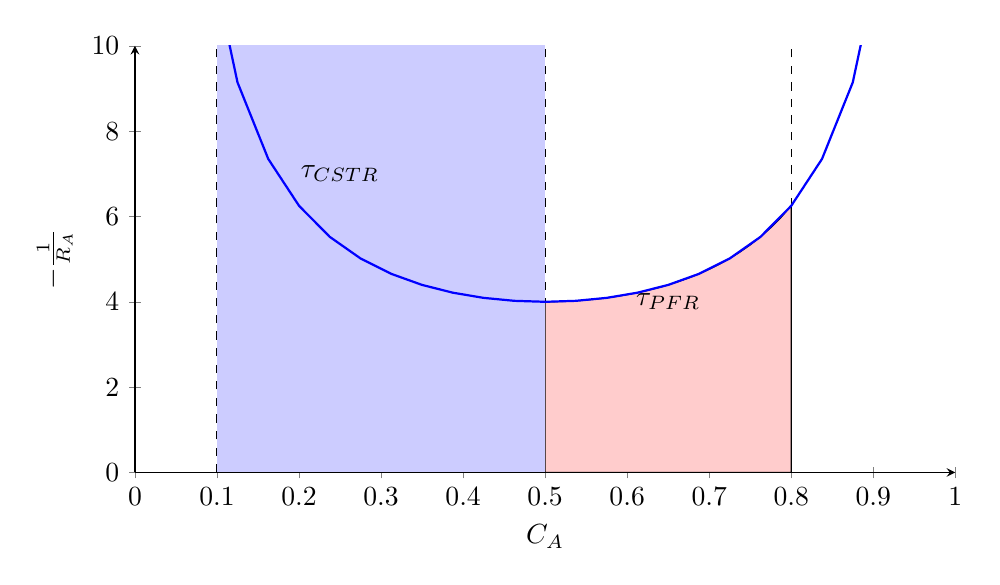
\begin{tikzpicture}
    \begin{axis}[
        width=12cm,
        height=7cm,
        xlabel={$C_A$},
        ylabel={$-\frac{1}{R_A}$},
        xmin=0, xmax=1,
        ymin=0, ymax=10,
        axis lines=left,
        domain=0.05:0.95]
    % parameters
    \def\k{1}
    \def\CAzero{1}
    % concentraties
    \def\CAin{0.8}
    \def\CAstar{0.5}
    \def\CAout{0.1}
    % verticale lijnen
    \addplot[dashed] coordinates {(\CAin,0) (\CAin,10)};
    \addplot[dashed] coordinates {(\CAstar,0) (\CAstar,10)};
    \addplot[dashed] coordinates {(\CAout,0) (\CAout,10)};
    % PFR oppervlakte (eerst)
    \addplot[fill=red!20,domain=\CAstar:\CAin]
    {1/(\k*x*(\CAzero-x))} \closedcycle;
    % CSTR rechthoek (nadien)
    \addplot[fill=blue!20,draw=none]
    coordinates {
    (\CAstar,0)
    (\CAout,0)
    (\CAout,{1/(\k*\CAout*(\CAzero-\CAout))})
    (\CAstar,{1/(\k*\CAout*(\CAzero-\CAout))})};
    \node at (axis cs:0.65,4) {$\tau_{\text{PFR}}$};
    \node at (axis cs:0.25,7) {$\tau_{\text{CSTR}}$};
    % curve
    \addplot[thick,blue]
    {1/(\k*x*(\CAzero-x))};
    \end{axis}
    \end{tikzpicture}
    \end{solution}
\end{question}
\begin{question}
Bepaal het benodigde volume van een serieschakeling van één CSTR en één PFR met een intermediaire concentratie $C_A^* = 0.5\ \text{kmol/m}^3$ en een eindconversie $X_A = 99\%$.

$V_1 = \answer{13.2}\ \text{m}^3$

$V_2 = \answer{30.4}\ \text{m}^3$
    
\begin{hint}
Bereken eerst het volume van de CSTR met
\[
\tau_1 = \frac{V_1}{q} = \frac{C_{A0}-C_A^*}{k\,C_A^*(C_{A0}-C_A^*)}.
\]
Voor de PFR gebruik je
\[
\tau_2 = \frac{V_2}{q} = -\int_{C_A^*}^{C_{A,\text{uit}}} 
\frac{dC_A}{k\,C_A(C_{A0}-C_A)}.
\]
Splits de breuk met partieelbreuken.
\end{hint}

\begin{solution}

\textbf{CSTR}

\[
\tau_1 = \frac{V_1}{q}
= \frac{C_{A0}-C_A^*}{k\,C_A^*(C_{A0}-C_A^*)}
= 1.32\ \text{uur}
\]

\[
V_1 = 13.2\ \text{m}^3
\]

\textbf{PFR}

\[
\tau_2 = \frac{V_2}{q}
= -\int_{C_A^*}^{C_{A,\text{uit}}} 
\frac{dC_A}{k\,C_A(C_{A0}-C_A)}
\]

\[
= -\frac{1}{kC_{A0}} 
\int_{C_A^*}^{C_{A,\text{uit}}} 
\left(
\frac{1}{C_A} + \frac{1}{C_{A0}-C_A}
\right) dC_A
= 3.04\ \text{uur}
\]

\[
V_2 = 30.4\ \text{m}^3
\]

\end{solution}
\end{question}
\end{exercise}

\begin{question}
    Evaluate the following:
    \begin{enumerate}
        \item $|2-5| = \answer{3}$
        \item $|5-2| = \answer{3}$
        \item $|5-\sqrt{2}| = \answer{5-\sqrt{2}}$
        \item $|5-\sqrt{2}| = \answer{3.58578643763}$
    \end{enumerate}
    If $x > 3$ then:
    \begin{enumerate}
        \item $|x - 3| = \answer{x - 3}$
        \item $|3 - x| = \answer{x - 3}$
        \item $|\sin(x) - 3| = \answer{3 - \sin(x)}$
    \end{enumerate}
\end{question}



\end{document}